% !TEX root =../thesis-letomes.tex

\chapter{Miscellaneous Derivations}

\section{Nondimensionalization of H-R4B Equations of Motion} \label{apx:hr4b-nondimensionalization}

Looking at the \(p_j\) from \cref{eq:pr,eq:ptheta,eq:pphi} we can infer their units:

\begin{align}
    k_{pr} &= \frac{k_m}{k_r k_t} \\[0.2cm]
    k_{p\theta} &= \frac{k_m k_r^2}{k_t} = k_{pr} k_r \\[0.2cm]
    k_{p\phi} &= k_{p\theta}
\end{align}

We now introduce the quantity

\begin{equation}
    b_j = \frac{p_j}{m_s}.
\end{equation}
It proves useful to introduce into Hamilton's equations because the mass cancels out (as expected from Newton's 2nd Law, and thus removes the need for introducing  selecting characteristic mass \(k_m\). We will treat the interpretation later. \(b_j\) has units:

\begin{align}
    k_{br} = \frac{k_{pr}}{k_m} = \frac{k_r}{k_t} \\[0.2cm]
    k_{b\theta} = \frac{k_{p\theta}}{k_m} = \frac{k_r^2}{k_t} \\[0.2cm]
    k_{b\phi} = \frac{k_{p\phi}}{k_m} = \frac{k_r^2}{k_t}
\end{align}

For the \(q_j\), \cref{eq:rdot,eq:thetadot,eq:phidot}, we set \(b_j = \frac{p_j}{m_s}\) and nondimensionalize:

\begin{align}
    \od{r}{t} &= \frac{\blue{p_r}}{\blue{p_r}} \\[0.2cm]
    \Leftrightarrow \od{r}{t} &= \blue{b_r} \\[0.2cm]
    \Leftrightarrow \frac{k_r}{k_t} \od{R}{T} &= k_{br} B_R,
\end{align}
so we get
\begin{empheq}[box=\widefbox]{align}
    \label{eq:Rdot}
    \dot{R} = B_R
\end{empheq}

\begin{align}
    \od{\theta}{t} &= \frac{\blue{p_\theta}}{\blue{m_s} r^2} \\[0.2cm]
    \Leftrightarrow \od{\theta}{t} &= \frac{\blue{b_\theta}}{r^2} \\[0.2cm]
    \Leftrightarrow \od{\theta}{t} &= \frac{b_\theta}{r^2} \\[0.2cm]
    \Leftrightarrow \frac{1}{k_t} \od{\theta}{T} &= \frac{k_{b\theta}}{k_r^2} \frac{B_\theta}{R^2},
\end{align}
so we get
\begin{empheq}[box=\widefbox]{align}
    \label{eq:thetadot-nondim}
    \dot{\theta} = \frac{B_\theta}{R^2}
\end{empheq}

\begin{align}
    \od{\phi}{t} &= \frac{\blue{p_\phi}}{{\blue{m_s}} r^2 \sin^2{\theta}} \\[0.3cm]
    \Leftrightarrow \od{\phi}{t} &= \frac{\blue{b_\phi}}{r^2 \sin^2{\theta}}  \\[0.3cm]
    \Leftrightarrow \frac{1}{k_t} \frac{\Phi}{T} &= \frac{k_\phi}{k_r^2} \frac{B_\phi}{R^2 \sin^2{\theta}},
\end{align}
so we get
\begin{empheq}[box=\widefbox]{align}
    \label{eq:phidot-nondim}
    \dot{\phi} = \frac{B_\phi}{R^2 \sin^2{\theta}}
\end{empheq}

For the \(p_j\), \cref{eq:prdot,eq:pthetadot,eq:pphidot} , we first divide by \(m_s\) then set \(b_j = \frac{p_j}{m_s}\) (\blue{relevant terms marked in blue}) and \(\mu_k = G M_k\):

\begin{align}
    \begin{split}
        \od{\blue{p_r}}{t} = -\pd{H}{q_r} &= \frac{\blue{p_\theta^2}}{\blue{m_s} r^3} + \frac{\blue{p_\phi^2}}{\blue{m_s} r^3 \sin^2{\theta} } \\
        &+ G \blue{m_s} \\
        &\sum\limits_{k} M_k \frac{-r + r_k \left(\cos{\theta}\cos{\theta_k} + \sin{\theta}\sin{\theta_k}\cos{(\phi - \phi_k)}\right)}{\left[r^2 + r_k^2 - 2 r r_k \left(\cos{\theta}\cos{\theta_k} + \sin{\theta}\sin{\theta_k}\cos{(\phi - \phi_k)} \right) \right]^{3/2}},
    \end{split} \\[0.3cm]
    \begin{split}
        \Leftrightarrow \od{\blue{b_r}}{t} &= \frac{\blue{b_\theta^2}}{r^3} + \frac{\blue{b_\phi^2}}{r^3 \sin^2{\theta} } \\
        &+ \sum\limits_{k} \mu_k \frac{-r + r_k \left(\cos{\theta}\cos{\theta_k} + \sin{\theta}\sin{\theta_k}\cos{(\phi - \phi_k)}\right)}{\left[r^2 + r_k^2 - 2 r r_k \left(\cos{\theta}\cos{\theta_k} + \sin{\theta}\sin{\theta_k}\cos{(\phi - \phi_k)} \right) \right]^{3/2}}.
    \end{split}
\end{align}
And finally we nondimensionalize:
\begin{align}
    \begin{split}
        \Leftrightarrow \teal{\frac{k_{br}}{k_t}} \od{B_R}{T} &= \orange{\frac{k_{b\theta}^2}{k_r^3}} \frac{B_\theta^2}{R^3} + \orange{\frac{k_{b\phi}^2}{k_r^3}} \frac{B_\phi^2}{R^3 \sin^2{\theta} } \\
        &+ \red{\frac{k_r^3}{k_t^2}\frac{1}{k_r^2}} \\
        & \sum\limits_{k} \eta_k \frac{-R + R_k \left(\cos{\theta}\cos{\theta_k} + \sin{\theta}\sin{\theta_k}\cos{(\phi - \phi_k)}\right)}{\left[R^2 + R_k^2 - 2 R R_k \left(\cos{\theta}\cos{\theta_k} + \sin{\theta}\sin{\theta_k}\cos{(\phi - \phi_k)} \right) \right]^{3/2}},
    \end{split}
\end{align}

where the characteristic units are colored teal, orange and red, \([\mu] = [G] [M_k] = \frac{k_r^3}{k_m k_t^2} k_m = \frac{k_r^3}{k_t^2} \), the first part of the red factor, the second part being from the fraction inside the summation, having units \(\frac{1}{k_r^2}\). Dividing \(\frac{k_{br}}{k_t}\) over from the left-hand side the units cancel as they must:

\begin{align}
    & \teal{\frac{k_t}{k_{br}}} \orange{\frac{k_{b\theta}^2}{k_r^3} } \\
    = &\frac{k_t^2}{k_r} \frac{k_r^4}{k_t^2 k_r^3}\\
    = &1,
\end{align}
and equivalently same for the second orange since \(k_\theta\) and \(k_\phi\) have the same units. And the red terms:

\begin{align}
    & \teal{\frac{k_t}{k_{br}}} \red{\frac{k_r^3}{k_t^2}\frac{1}{k_r^2}} \\
    = &\frac{k_t^2}{k_r} \frac{k_r^3}{k_t^2} \frac{1}{k_r^2} \\
    = &1
\end{align}

and we are left with the nondimensionalized equation:
\begin{empheq}[box=\widefbox]{align}
    \label{eq:Brdot}
    \dot{B}_r = &\frac{B_\theta^2}{R^3} + \frac{B_\phi^2}{R^3 \sin^2{\theta}} \\
    & + \sum\limits_{k} \eta_k \frac{-R + R_k \left(\cos{\theta}\cos{\theta_k} + \sin{\theta}\sin{\theta_k}\cos{(\phi - \phi_k)}\right)}{\left[R^2 + R_k^2 - 2 R R_k \left(\cos{\theta}\cos{\theta_k} + \sin{\theta}\sin{\theta_k}\cos{(\phi - \phi_k)} \right) \right]^{3/2}} \notag
\end{empheq}

The exact same procedure for \(\dot{p_\theta}\) and \(\dot{p}_\phi\) gives us:

\begin{empheq}[box=\widefbox]{align}
    \label{eq:Bthetadot}
    \dot{B}_\theta = &\frac{B_\phi^2}{R^2 \sin^2{\theta} \tan{\theta}} \\
    &+ \sum\limits_{k} \eta_k \frac{R R_k \left[-\sin{\theta}\cos{\theta_k} + \cos{\theta}\sin{\theta_k}\cos{(\phi - \phi_k)} \right]}{\left[R^2 + R_k^2 - 2 R R_k \left(\cos{\theta}\cos{\theta_k} + \sin{\theta}\sin{\theta_k}\cos{(\phi - \phi_k)} \right) \right]^{3/2}} \notag
\end{empheq}

\begin{empheq}[box=\widefbox]{align}
    \label{eq:Bphidot}
    \dot{B}_\phi = &\sum\limits_{k} \eta_k \frac{- R R_k \sin{\theta}\sin{\theta_k}\sin{(\phi - \phi_k)}}{\left[R^2 + R_k^2 - 2 R R_k \left(\cos{\theta}\cos{\theta_k} + \sin{\theta}\sin{\theta_k}\cos{(\phi - \phi_k)} \right) \right]^{3/2}}
\end{empheq}

Finally we can get the nondimensionalize \(H\) by the same method. Again we first divide by \(m_s\) to obtain ``Hamiltonian per spacecraft mass'', \(H/m_s = H_m\):

\begin{equation*}
    \begin{aligned}
        H &= \frac{p_r^2}{2 m_s} + \frac{p_\theta^2}{2 m_s r^2} + \frac{p_\phi^2}{2 m_s r^2 \sin^2{\theta}} \\
        &- G m_s \sum\limits_{k} \frac{M_k}{\sqrt{r^2 + r_k^2 - 2 r r_k \left[\cos{\theta}\cos{\theta_k}+\sin{\theta}\sin{\theta_k}\cos{(\phi - \phi_k})\right]}},
    \end{aligned}
\end{equation*}

\begin{equation}
    \begin{aligned}
        \Leftrightarrow H_m &= \frac{b_r^2}{2} + \frac{b_\theta^2}{2 r^2} + \frac{b_\phi^2}{2 r^2 \sin^2{\theta}} \\
        &- \sum\limits_{k} \mu_k \frac{1}{\sqrt{r^2 + r_k^2 - 2 r r_k \left[\cos{\theta}\cos{\theta_k}+\sin{\theta}\sin{\theta_k}\cos{(\phi - \phi_k})\right]}},
    \end{aligned}
\end{equation}

and then use our characteristic units to get \(\mathcal{H}_m\):

\begin{equation}
    \begin{aligned}
        \Leftrightarrow \mathcal{H}_m &= \frac{B_r^2}{2} + \frac{B_\theta^2}{2 R^2} + \frac{B_\phi^2}{2 R^2 \sin^2{\theta}} \\
        &- \sum\limits_{k} \eta_k \frac{1}{\sqrt{R^2 + R_k^2 - 2 R R_k \left[\cos{\theta}\cos{\theta_k}+\sin{\theta}\sin{\theta_k}\cos{(\phi - \phi_k})\right]}}. \label{eq:HH_m}
    \end{aligned}
\end{equation}

\section{Symplectic Verlet Derivations}\label{apx:symplectic-verlet-derivations}

\subsection{Symplectic Verlet Derivations (Handwritten)}
\includepdf[scale=1.0,pages={-}]{pdf/r4b-symplectic-verlet-handwritten.pdf}

\subsection{Symplectic Verlet Derivations (Mathematica Check)}
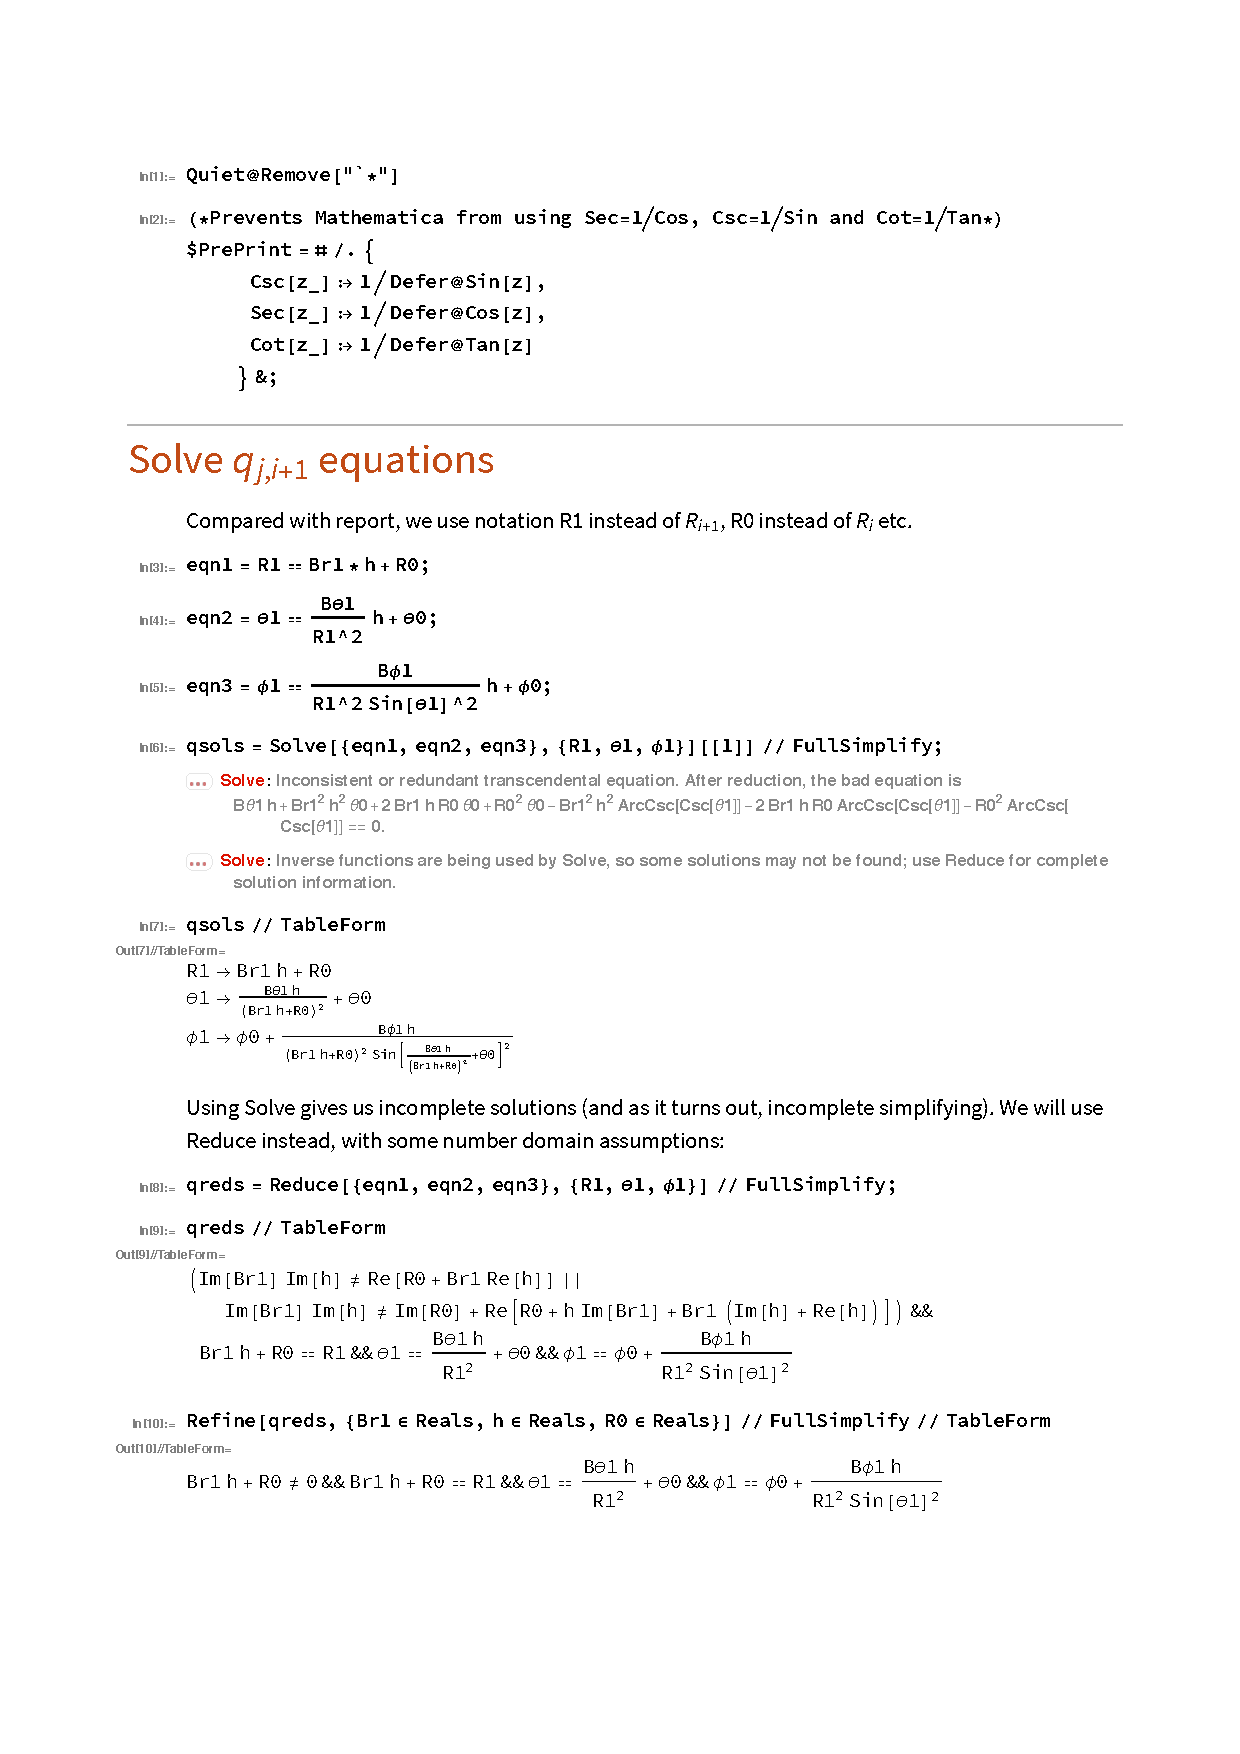
\includepdf[scale=1.0,pages={-}]{pdf/r4b-symplectic-verlet-mathematica.pdf}